% So we make this "beamer" rather than document!

\documentclass[11pt]{beamer}
% For handout add ,handout after 11pt
% Kill page numbers with [numbering=none] in next line:
\usetheme[sectionpage=none,numbering=none]{metropolis}           % Use metropolis theme
	% To do printouts, add ", handout"  after aspectratio.
\usepackage{makecell}
\usepackage{booktabs}
\usepackage{graphicx}
\usepackage{color}
%\usepackage[utf-8]{inputenc}
\usepackage{bbm}
  \usepackage{bm}
\newcommand{\notimplies}{%
  \mathrel{{\ooalign{\hidewidth$\not\phantom{=}$\hidewidth\cr$\implies$}}}}
\definecolor{violet}{RGB}{223,115,255}
\usepackage{transparent}
\definecolor{cyan2}{RGB}{0,255,255}
\makeatletter
\newcommand\primitiveinput[1]
{\@@input #1 }
\makeatother
\usepackage{tabu}
\usepackage{dcolumn}
\definecolor{Gray}{gray}{0.85}

\usepackage{xcolor,colortbl}


\title{Practical Data Science I: \\ Wrangling Data and Answering Questions}
\author{\small Adriane Fresh \& Nick Eubank}
\date{\vspace*{.3in} \date}


% This is the beginning of a real document!
\begin{document}

\begin{frame}
\maketitle
\end{frame}


\begin{frame}[c]{What is Data Science?}
\begin{enumerate}
	\pause \item What (\alert{in theory}) do we think Data Science should be?
	\pause \item What (\alert{empirically}) is Data Science?
\end{enumerate}
\end{frame}


\begin{frame}[c]{What (in theory) should Data Science be?}

\pause Study of how to \alert{solve problems} \pause by \alert{answering questions} \pause using \alert{quantitative data.}

\pause
\begin{itemize}
	\item Problem-first approach. 
	\begin{itemize}
		\pause \item Data Science is an \emph{applied} discipline!
	\end{itemize} 
	\pause \item The tool you use should be dictated by the question you seek to answer
\end{itemize}

\end{frame}


\begin{frame}[c]{What (empirically) is Data Science?}

\end{frame}

\begin{frame}[c]{How did Data Science become a thing?}

Over the past several decades:
\begin{enumerate}
	\item Availability of data $\uparrow$
	\item Computational power $\uparrow$
\end{enumerate}
\pause
$\Rightarrow$ Huge proliferation and increase in sophistication of computational methods
\end{frame}


\begin{frame}[c]{How did Data Science become a thing?}

\begin{itemize}
	\item Academic research is organized into silos:
	\pause
	\begin{itemize}
		\item Computer Science
		\item Statistics
		\item Economics
		\item Political science
		\item Engineering
	\end{itemize}
\end{itemize}
\pause $\Rightarrow$ Development of new tools occurred \emph{within} each silo.
\end{frame}


\begin{frame}[c]{Where are we today?}
Very little cross-pollination across silos
\begin{itemize}
	\pause \item Lots of duplication of development.
	\pause \item Every silo has its own vocabulary.
	\pause \item Each silo has focused on the aspects most relevant to their applications. e.g.:
	\begin{itemize}
		\pause \item CS likes to classify things and make predictions, don't care how model works
		\item Social scientists like to make causal statements, don't care about predictive power
	\end{itemize}
\end{itemize}
\end{frame}

\begin{frame}[c]{}
\pause 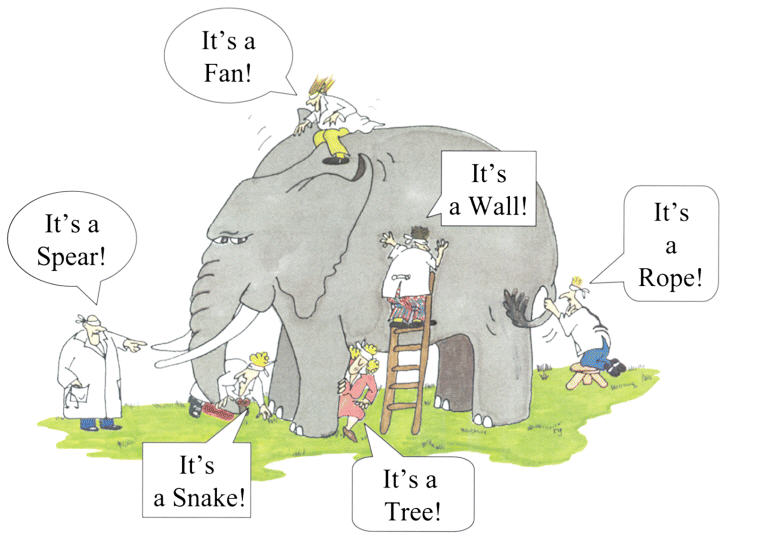
\includegraphics[width=\textwidth]{blindmenelephant.jpg}
\pause $\Rightarrow$ This is where we are \emph{now.}
\end{frame}

\begin{frame}[c]{What is (empirically) Data Science?}
\pause An effort to unify the development of quantitative methods \\
\pause $\rightarrow$ Recognize the elephant
\end{frame}

\begin{frame}[c]{Why does this matter to you?}
\begin{itemize}
	\item Most current researchers learned their skills in a silos. \\
	\pause In many ways, \alert{\emph{you} will have better perspective than your professors.}
	\pause \item Expect fragmentation in both software and vocabulary. \\
	\pause The fact things don't always seem coherent isn't because you're missing something.
\end{itemize}
\end{frame}


\begin{frame}[c]{Why does this matter to you?}
\begin{itemize}
	\item Many of you will have a conception of what is (and is not) data science.
	\begin{itemize}
		\pause \item Don't hold to those beliefs too strongly.
	\end{itemize}
	\pause \item My people who talk about data science were trained in a single silo, and may not fully recognize what's happening beyond.
	\begin{itemize}
		\pause \item That's why we have faculty from many fields.
	\end{itemize}
\end{itemize}
\end{frame}

\begin{frame}[c]{This Class}

``The Python Class'' \\

\begin{itemize}
	\pause \item \emph{Data Science} Python
	\begin{itemize}
		\pause \item Python standard library, numpy, pandas, scikit-learn, matplotlib, statsmodels
	\end{itemize}
\end{itemize}
\end{frame}

\begin{frame}[c]{``The Everything-That-Comes-\emph{Before}-Data-Analysis Class''}

\pause In this course, you will learn:
\begin{itemize}
	\pause \item Think computationally,
	\pause \item Write your own algorithms and generalized code,
	\pause \item about different data formats and how to work with them,
	\pause \item to work with real, messy, error-ridden data,
	\pause \item best practices for data science workflow management and collaboration.
\end{itemize}
\pause \alert{All} through hands-on experience.
\end{frame}

\begin{frame}[c]{This Class}

	So yes, we will be working \emph{in} Python, \\ 
\pause but this isn't a class \emph{about} Python. \\
\pause $\Rightarrow$ Emphasis on generalizable data science skills

\end{frame}

\begin{frame}[c]{This Class}
By the end of this class:
\begin{itemize}
	\pause \item Find and organize data \emph{on your own}.
	\pause \item Understand how to clean, merge, and manipulate real-world data.
	\pause \item Know how to approach organizing a full project.
\end{itemize}
\end{frame}


\begin{frame}{Why Python?}
\pause And why not:
\begin{itemize}
	\item Stata \\ 
	\uncover<3->{Excellent for tabular data, some text}
	\item R (Tidy-Verse)\\ 
	\uncover<4->{Excellent for tabular data}
	\item R (Base-R) \\
	\uncover<4->{Good for tabular, network, geospatial, some text and ML}
\end{itemize}
?
\end{frame}

\begin{frame}{Why Python?}
Python:
\begin{itemize}
	\item Tabular data
	\item Network data
	\item Geospatial data
	\item Natural Language Processing (NLP)
	\item Neural Networks
	\item Using with Cloud Compute
	\item Big Data
	\item Large Language Models
	\item All Machine Learning
	\item ...
\end{itemize}
\end{frame}

\begin{frame}[c]{Why?}

Language Intrinsics:
\begin{itemize}
	\pause \item R and Stata are \emph{domain-specific languages} (DSLs).
	\begin{itemize}
		\pause \item Simplified to make them easier for researchers to start using.
	\end{itemize}
	\pause \item Python is a \emph{general purpose language}.
	\begin{itemize}
		\pause \item Python is foundational at OpenAI, Instagram, Dropbox, Netflix.
	\end{itemize}
\end{itemize}

\pause Network Effects:
\begin{itemize}
	\pause \item 90s and 2000s (even 2010s): most social scientists used Stata or R, developed for Stata and R.
	\pause \item 2010s and 2020s: Businesses, computer scientists and software engineers moved to data science.
	\begin{itemize}
		\item Wanted a fully-featured, general purpose language (ideally one they know).
	\end{itemize}
\end{itemize}
\end{frame}


\begin{frame}[c]{Stack Overflow Developer Survey 2024}
		\centering

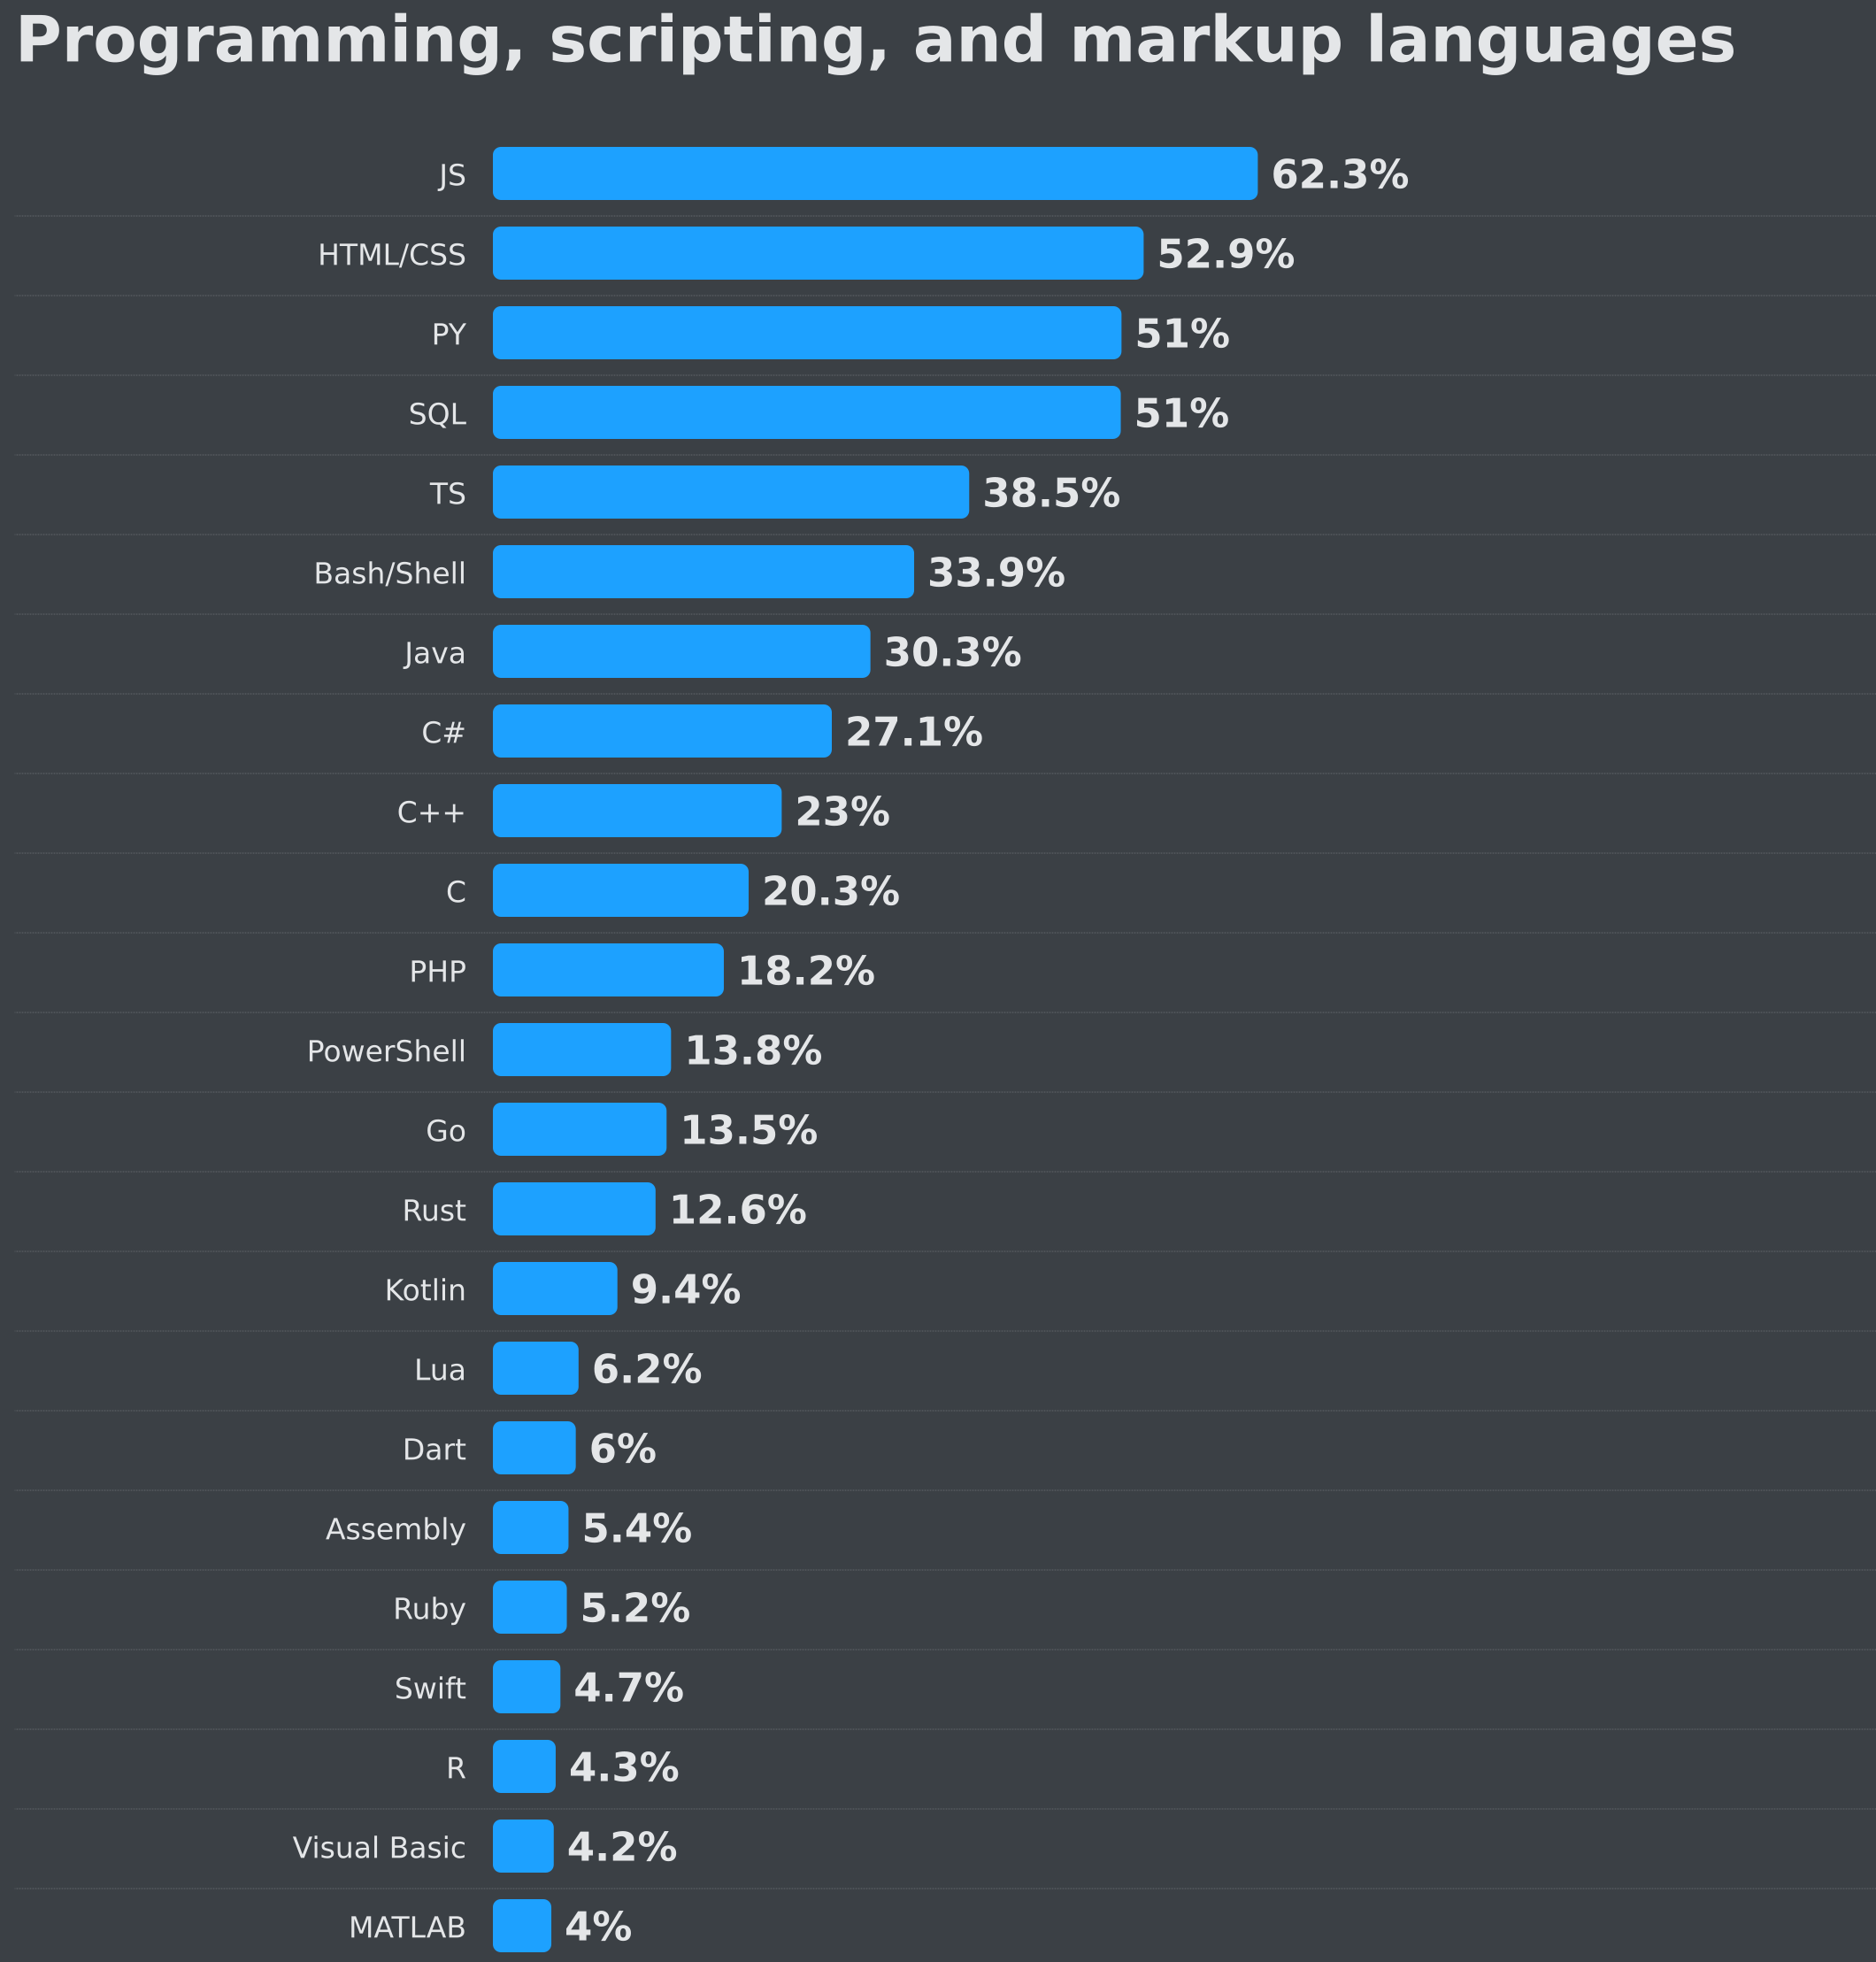
\includegraphics[width=0.7\textwidth]{stackoverflow2024_0.png}
\end{frame}

\begin{frame}[c]{Stack Overflow Developer Survey 2024}
	\centering

	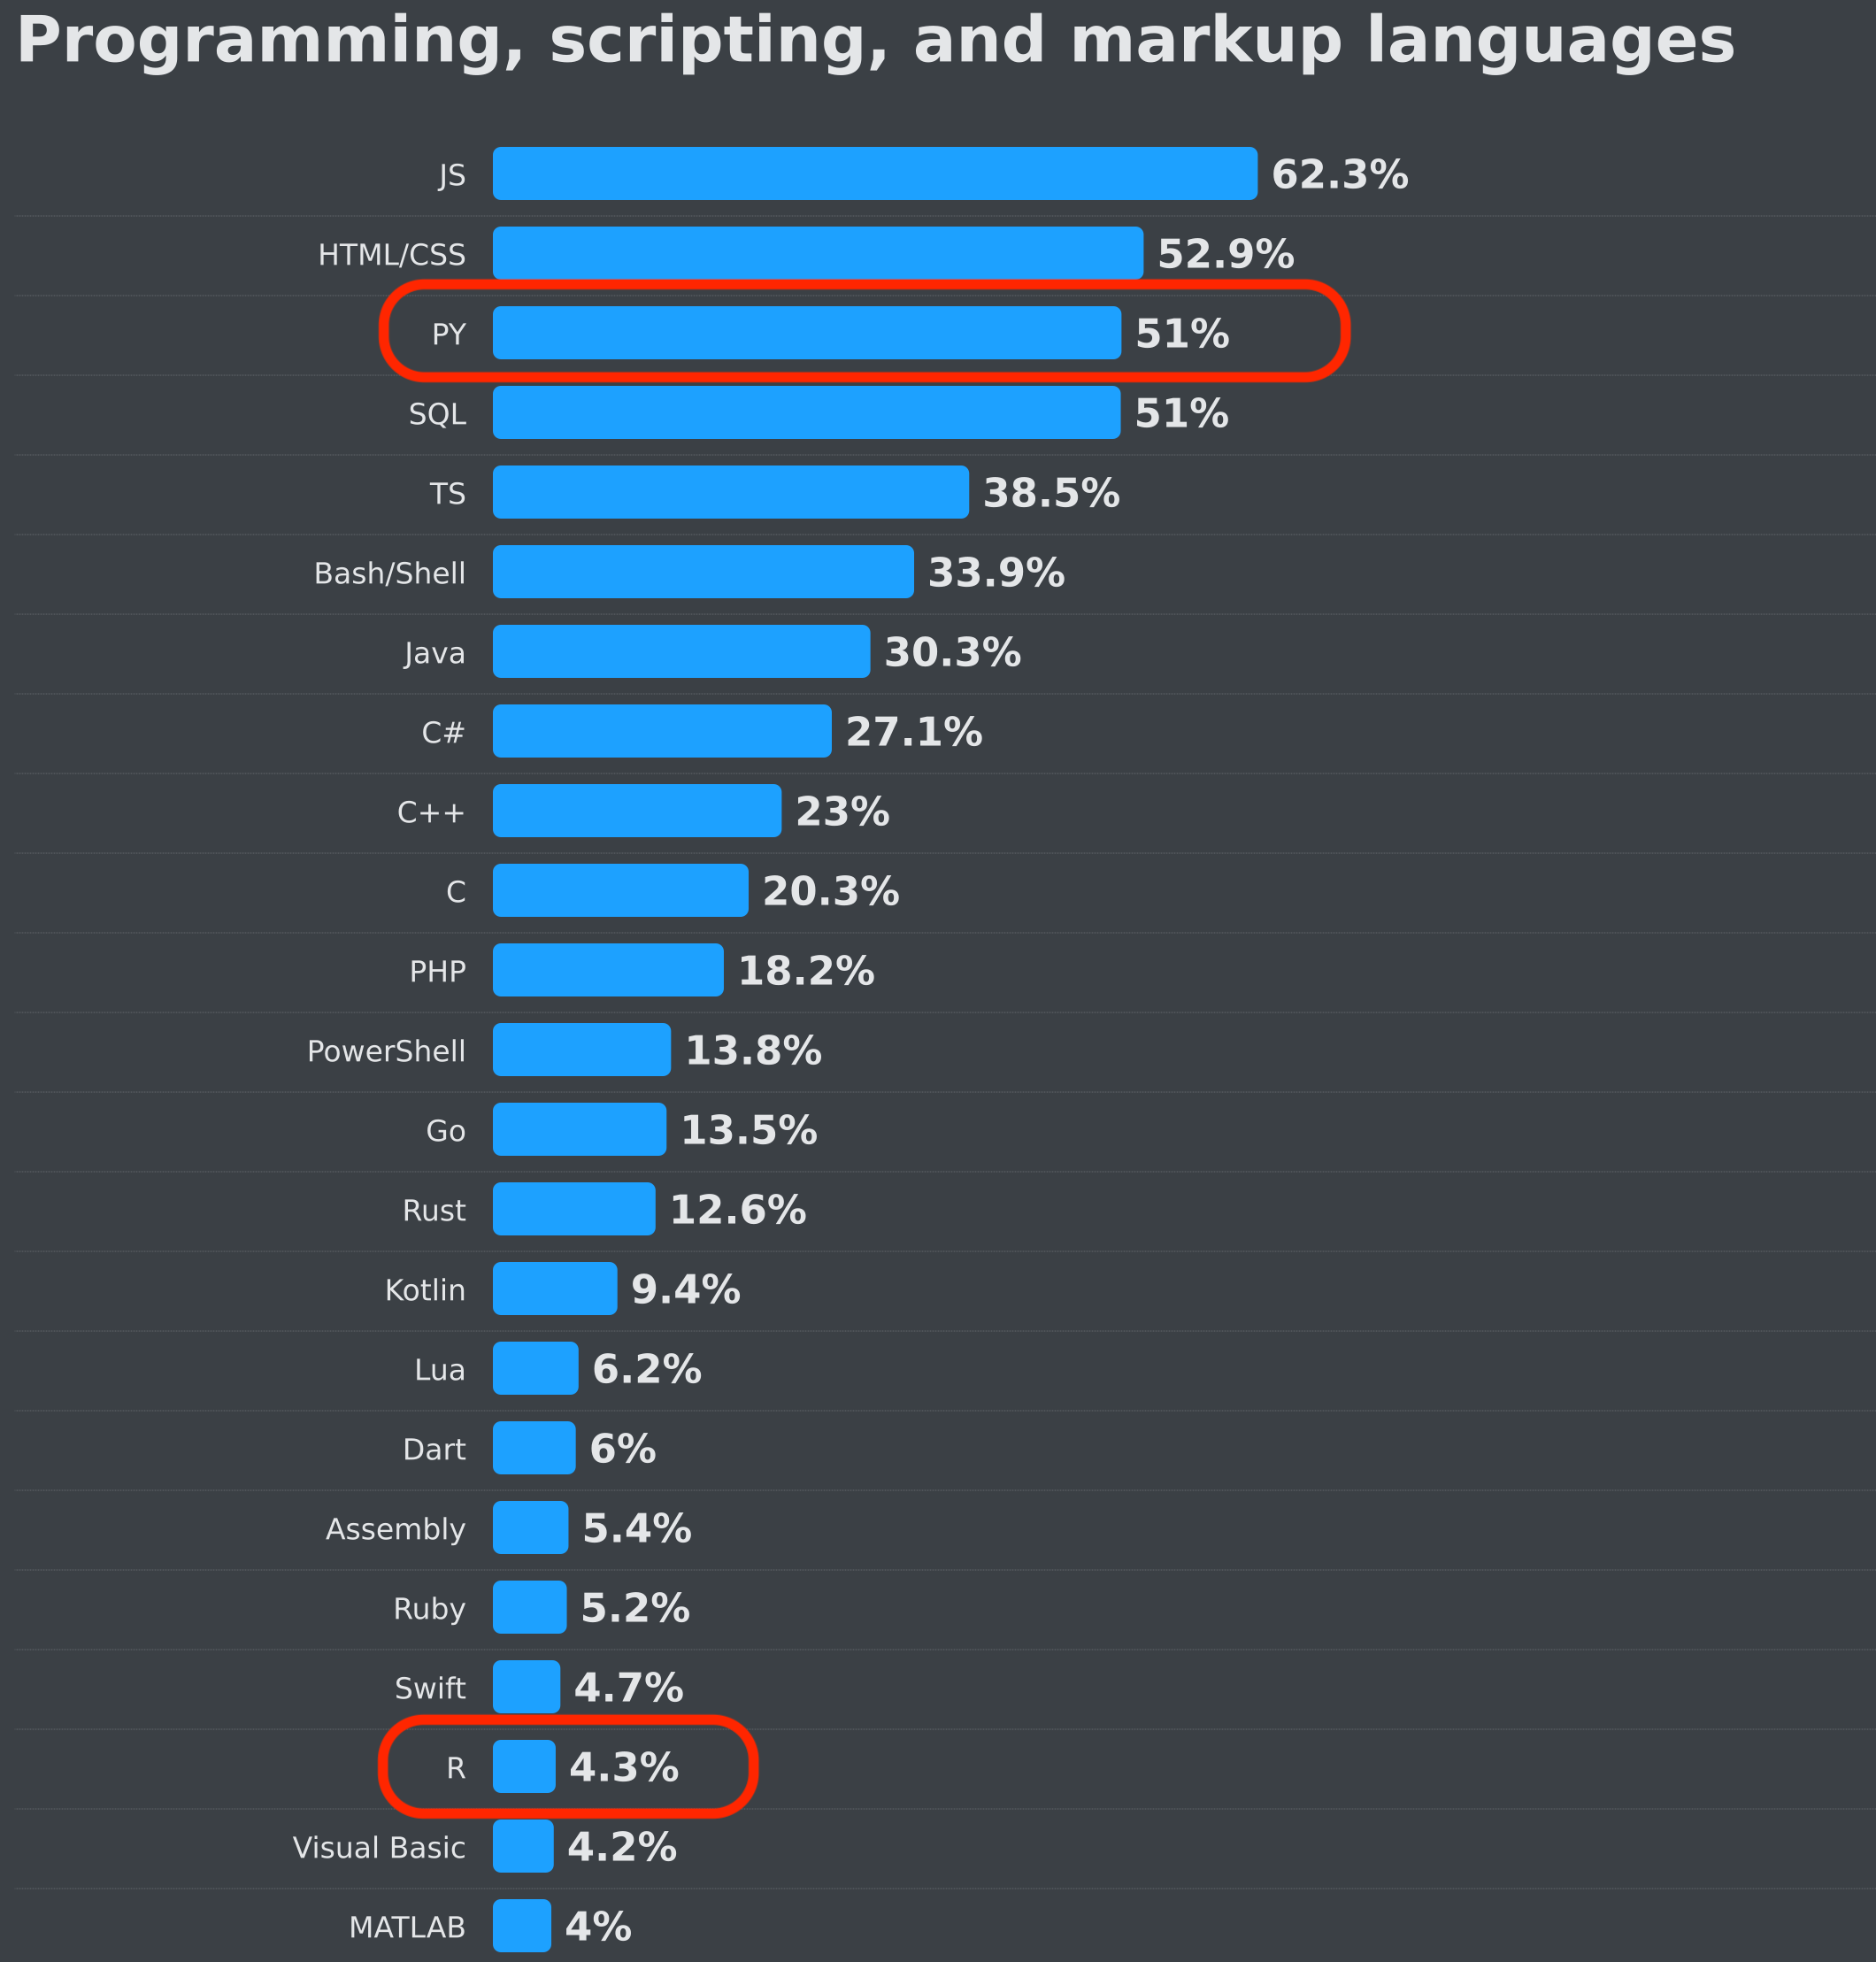
\includegraphics[width=0.7\textwidth]{stackoverflow2024_1.png}
\end{frame}


\begin{frame}[c]{}
	\centering
	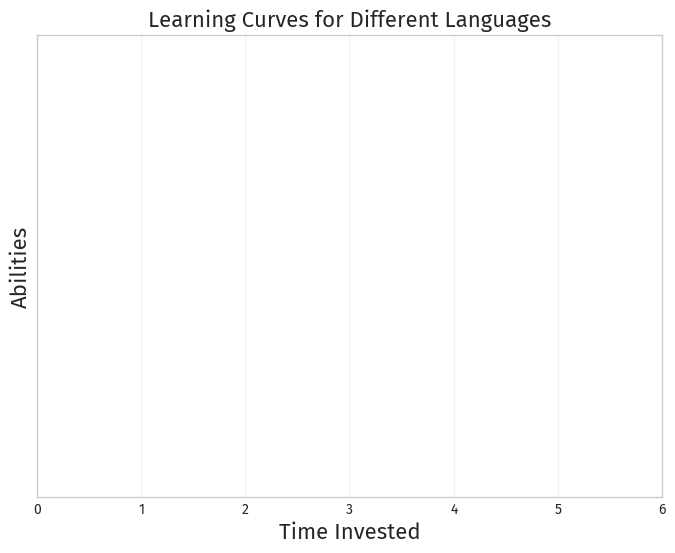
\includegraphics[width=\textwidth ]{language_0.png}
\end{frame}

\begin{frame}[c]{}
	\centering
	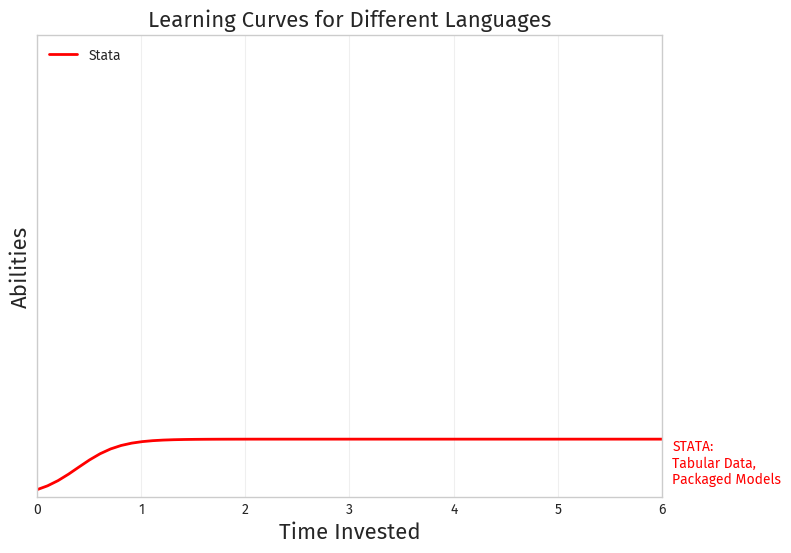
\includegraphics[width=\textwidth ]{language_1.png}
\end{frame}

\begin{frame}[c]{}
	\centering
	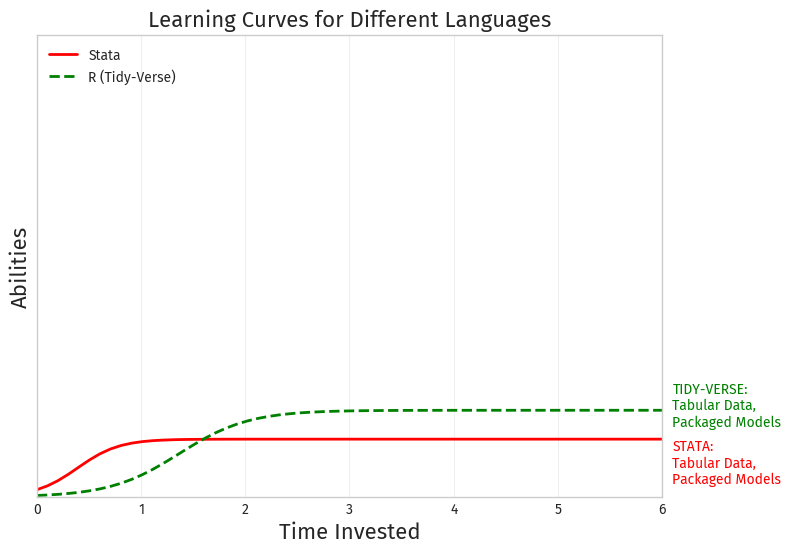
\includegraphics[width=\textwidth ]{language_2.png}
\end{frame}

\begin{frame}[c]{}
	\centering
	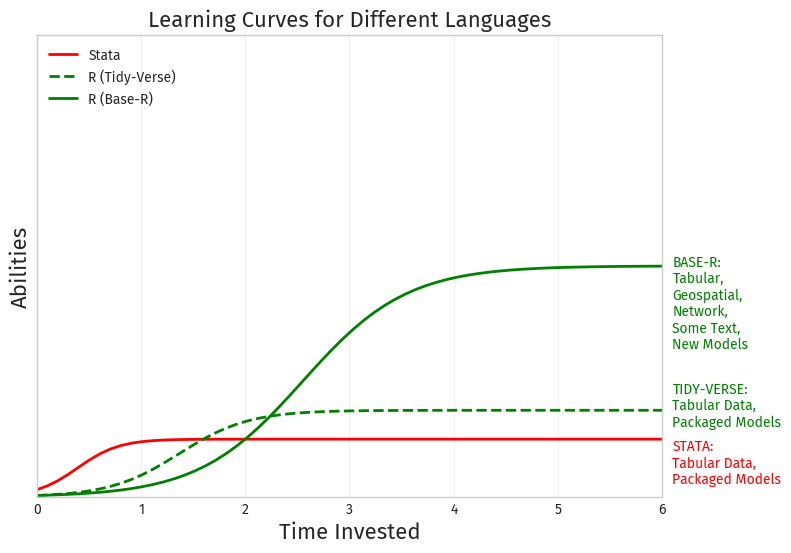
\includegraphics[width=\textwidth ]{language_3.png}
\end{frame}

\begin{frame}[c]{}
	\centering
	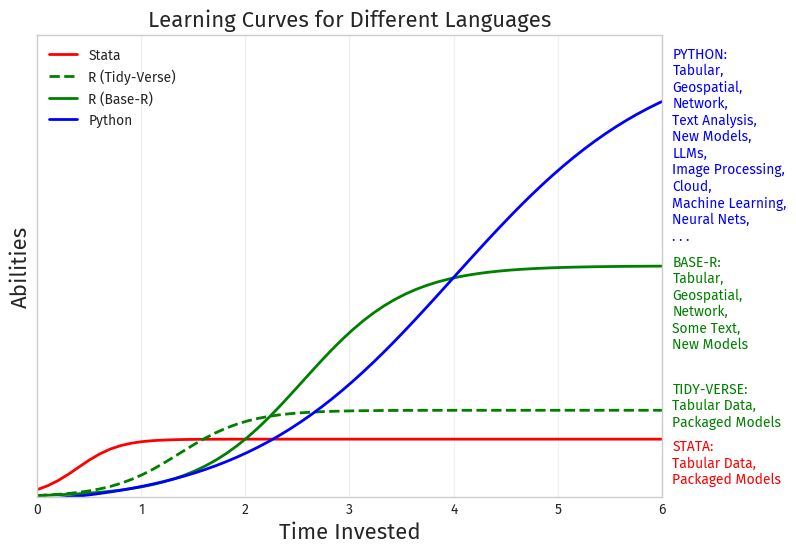
\includegraphics[width=\textwidth ]{language_4.png}
\end{frame}

\begin{frame}[c]{So what?}
\begin{itemize}
	\pause \item ``This is so much easier to do in [Stata/R]'' \\
	\begin{itemize}
		\item You're not wrong!
		\pause \item (Also easier ways in Python!)
	\end{itemize}
	\pause \item ``This isn't what I want to learn.''
	\begin{itemize}
		\item Especially for the first 4 weeks.
	\end{itemize}
\end{itemize}
\end{frame}

\begin{frame}[c]{By the end of this class...}
\begin{itemize}
	\item Manipulating and cleaning US census data,
	\pause \item Reshaping and aggregating arrest data,
	\pause \item Statistically estimating the effect of smoking on infant birthweight,
	\pause \item and more.
\end{itemize}
\end{frame}

\begin{frame}[c]{If you also take IDS 591...}
\begin{itemize}
	\item Work with big (terabyte sized) datasets,
	\pause \item Analyze geospatial satellite and demographic data,
	\pause \item Analyze social networks,
	\pause \item and more.
\end{itemize}
\end{frame}

\begin{frame}[c]{Most importantly, though...}
You will have a strong understanding of computational thinking and Python\\
\pause that will allow your empirical work to go wherever your research takes you, \\
\pause instead of feeling limited by what existing packages make easy.
\end{frame}

% \begin{frame}[c]{Areas of Data Science}
% 	\begin{columns}
% 	\begin{column}{0.45\textwidth}
% 		\uncover<1->{\textbf{Software Engineering DS}}
% 		\begin{itemize}
% 			\item \uncover<2->{Recommendation engines}
% 			\item \uncover<2->{Financial trading algorithms}
% 			\item \uncover<2->{Self-driving cars}
% 		\end{itemize}
% 	\end{column}
% 	\begin{column}{0.5\textwidth}  %%<--- here
% 		\uncover<1->{\textbf{Data Analysis DS}}
% 		\begin{itemize}
% 			\item \uncover<3->{Impact of policy change}
% 			\item \uncover<3->{Effectiveness of health interventions}
% 			\item \uncover<3->{Plan political campaigns}
% 		\end{itemize}
% 	\end{column}
% 	\end{columns}
% 	\vspace*{1cm}
% \uncover<4->{Nearly all data scientists will use some of both sets of skills.}\\
% \uncover<5->{In this class, we will be \emph{largely }focused on the \alert{Data Analysis} flavor of Data Science, but will touch on both.}
% \end{frame}

\begin{frame}[c]{About Us: Adriane Fresh}
	I am a scholar of political economy and political institutions \\
	\vspace{0.5cm}
	\begin{itemize}
		\pause \item PhD in Political Science
		\pause \item Master in Economics
		\pause \item BA in Economics and Latin American Studies, Minor in Math
	\end{itemize}
\end{frame}

\begin{frame}[c]{About Us: Adriane Fresh}
	Research:
	\begin{itemize}
		\pause \item Effects of economic and institutional changes on elite persistence and the strategies that elites.
		\pause \item I study a diverse set of historical time periods and country contexts including the Industrial Revolution in Britain, the enfranchisement of Black people in the U.S., regime change in Chile, and contemporary U.S. election administration. 
		\pause I am particularly interested in causal inference and natural language processing using large corpuses of historical and historiographical text.
	\end{itemize}
\end{frame}



\begin{frame}[c]{About Us: Nick Eubank}
	I am en empirical social scientist\\
	\vspace{0.5cm}
	\begin{itemize}
		\pause \item PhD in Political Economy
		\pause \item Master in Economics
		\pause \item BA in Economics and Political Science
	\end{itemize}
\end{frame}

\begin{frame}[c]{About Us: Nick Eubank}
	Research:
	\begin{itemize}
		\pause \item Looking for evidence of polling place manipulation in North Carolina
		\pause \item Developing methods of measuring Gerrymandering in the US.
		\pause \item Testing theories about how social networks shape political behavior using cell-phone meta-data to map social networks of entire countries (Zambia and Venezuela).
		\pause \item Studying whether political elites in the US South turned to using incarceration to prevent black voters from exercising political influence after the Voting Rights Act removed their ability to use Jim Crow restrictions.
	\end{itemize}
\end{frame}

\begin{frame}[c]{Features of this class}
\begin{itemize}
	\item Flipped Classroom
	\begin{itemize}
		\pause \item Need to come prepared,
		\pause \item Intermittent Reading Quizzes
	\end{itemize}
	\pause \item Lots of group work
	\begin{itemize}
		\pause \item Pair programming
		\pause \item You'll provide feedback to your partners
		\pause \item Don't start early
	\end{itemize}
	\pause \item Slack
	\pause \item Datacamp
	\pause \item Photos
\end{itemize}
\end{frame}


\begin{frame}[c]{}
	\begin{center}
www.practicaldatascience.org
	\end{center}
\end{frame}

\end{document}
